The normal vector to the ZOX plane is
\begin{align} 
\vec{n} = \myvec{0\\1\\0}.
\end{align}
Since, Y-axis has the intercept 3, the desired plane passes through the point
\begin{align}
\vec{P}=\myvec{0\\3\\0}.
\end{align}
Thus, the equation of the plane is given by,
\begin{align}
	\vec{n}^\top \brak{\vec{x}-\vec{P}} &= 0\\
	\implies \myvec{0&1&0} \vec{x}&= 3
\end{align}
See Fig. 
     \ref{fig:chapters/12/11/3/8/1}.
\begin{figure}[H]
  \centering
   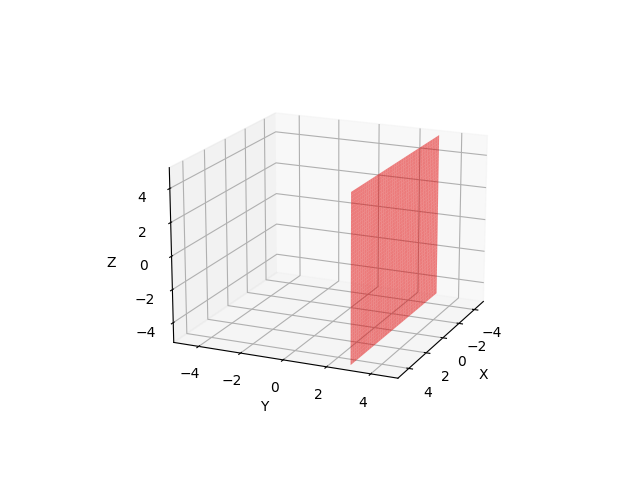
\includegraphics[width=0.75\columnwidth]{chapters/12/11/3/8/figs/plane1.png}
    \caption{}
     \label{fig:chapters/12/11/3/8/1}
     \end{figure}  
